\noindent Στο πρώτο ερώτημα της εργασίας καλούμαστε να υλοποιήσουμε στη GPU την 2D συνέλιξη ενός \mbox{μητρώου A}. Για τον υπολογισμό της νέας τιμής στη θέση (i,j) χρησιμοποιείται η τιμή της τρέχουσας θέσης καθώς και οι τιμές των οχτώ γειτονικών της, κάθε μία εκ των οποίων συνεισφέρει με ένα συγκεκριμένο βάρος στο τελικό αποτέλεσμα. Στο μητρώο Β, το οποίο αποθηκεύει τις υπολογισθείσες τιμές, για τις περιφερειακές (οριακές) θέσεις του πίνακα δεν γίνεται κάποιος υπολογισμός με αποτέλεσμα να συμπληρώνονται με μηδενικά.

\begin{center}
    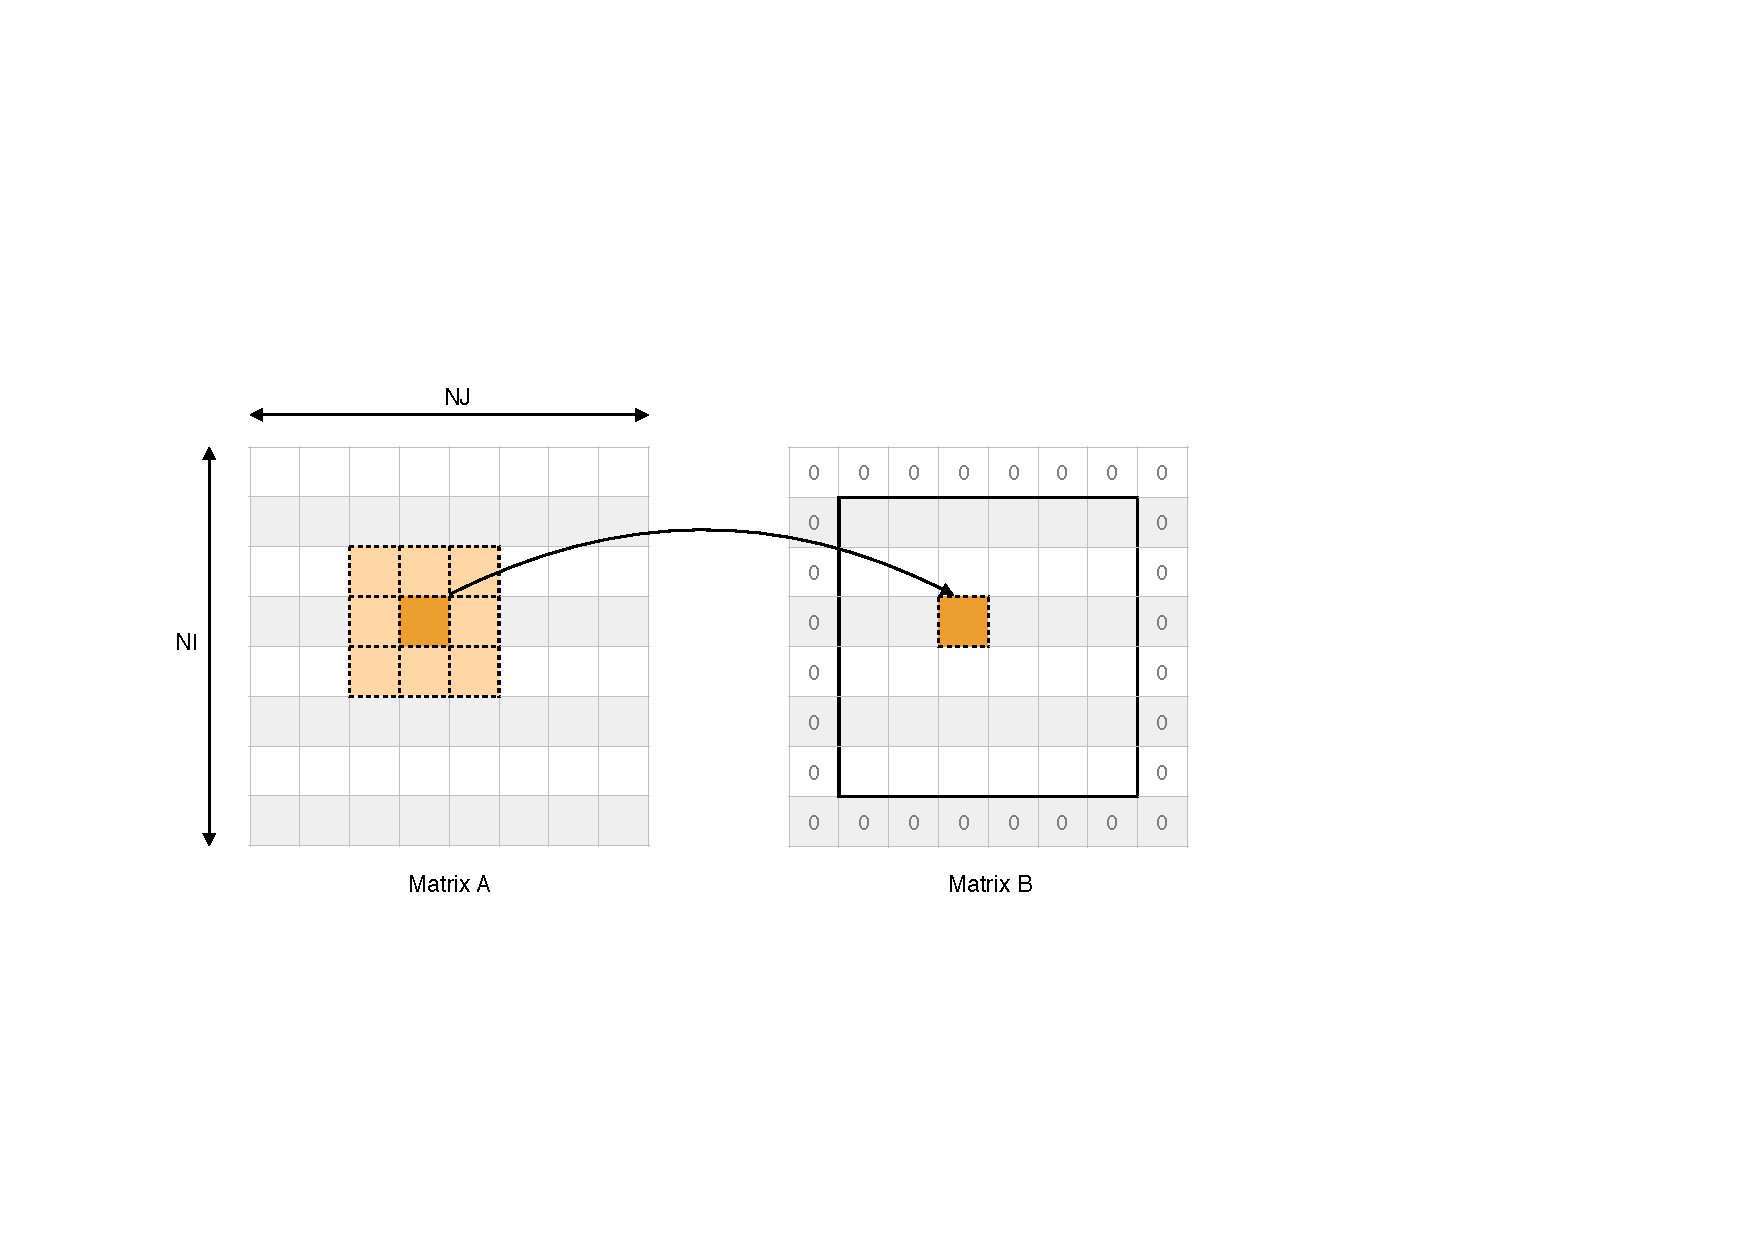
\includegraphics[scale=0.8]{./figures/1_conv/2d_conv}
\end{center}

\vspace{-0.8cm}
\subsection*{Πως όμως εξασφαλίζουμε την ορθότητα των υπολογισμών στη GPU;}
\addcontentsline{toc}{subsection}{Έλεγχος ορθότητας υπολογισμών}

Ένα ερώτημα που προκύπτει μετά την παραλληλοποίηση του κώδικα είναι αν έχει γίνει με σωστό τρόπο. Το γεγονός ότι εκτελείται χωρίς σφάλματα δεν μας εγγυάται την ορθότητα των υπολογισμών. Για την εξακρίβωσή της απαιτείται να καταστρώσουμε μια τεχνική ελέγχου η οποία θα μας διασφαλίζει ότι τελικά το μητρώο που υπολογίστηκε είναι το ζητούμενο. Σε μικρού μεγέθους προβλήματα ο οπτικός έλεγχος είναι εφικτός αφού μπορούμε να εκτυπώσουμε στην οθόνη τα αποτελέσματα και να τα αντιπαραβάλουμε με αυτά που προκύπτουν από τον αρχικό κώδικα. Με αυτόν τον τρόπο είναι πιο εύκολο να έχουμε μια πρώτη εικόνα του υπολογισμού μας η οποία μας επιτρέπει να ελέγξουμε με ευκολία τις οριακές περιπτώσεις, όπως τι συμβαίνει στα άκρα του μητρώου.

Για μεγαλύτερου μεγέθους προβλήματα αποφασίσαμε να ακολουθήσουμε μια τεχνική παρόμοια με αυτήν που παρουσιάστηκε στο μάθημα της Παράλληλης Επεξεργασίας κατά το προηγούμενο ακαδημαϊκό έτος. Συγκεκριμένα διατρέχουμε το μητρώο και αποθηκεύουμε είτε δειγματοληπτικά είτε το σύνολο των τιμών (όταν το μέγεθός του μας το επιτρέπει) σε ένα αρχείο. Κάνουμε το ίδιο και για τον αρχικό κώδικα και έπειτα τα συγκρίνουμε τα δύο αρχεία με χρήση της \texttt{numdiff}. Θεωρούμε ότι οι υπολογισμοί μας είναι ορθοί όταν οι τιμές που περιέχουν είναι ίσες (λαμβάνοντας υπόψιν ένα άνω όριο απόλυτου σφάλματος).

\vspace{-0.3cm}

\subsection*{Επιλογή μεγέθους block και grid}
\addcontentsline{toc}{subsection}{Επιλογή μεγέθους block και grid}

Το επόμενο θέμα που μας απασχόλησε είναι ποια είναι τα βέλτιστα μεγέθη block και grid για τα οποία παίρνουμε την καλύτερη απόδοση; Αφού το πρόβλημα μας περιέχει μητρώα δύο διαστάσεων, θα χρησιμοποιήσουμε δισδιάστατα block και grid. Τι μέγεθος όμως θα ορίσουμε σε κάθε μία από τις διαστάσεις για καθένα από αυτά τα δύο στοιχεία; Κάποια στοιχεία που πρέπει να ληφθούν υπόψιν περιγράφονται παρακάτω:

\begin{itemize}
    \item Το μέγεθος κάθε block δεν πρέπει να ξεπερνά τα 1024 threads με μέγιστες διαστάσεις (1024, 1024, 64).
    \item Κάθε block δεν μπορεί να καταναλώνει περισσότερους από 32k καταχωρητές.
    \item Κάθε block δεν μπορεί να καταναλώνει περισσότερο από 48kb shared memory.
    \item Ιδανικά, ο αριθμός των thread ανα block πρέπει να είναι πολλαπλάσιο του warp size (32 threads).
    H Tesla C2075 έχει 1.536 thread slots per SM. Αφού 1.536 = 32 × 48, έχουμε \#thread slots = warp size × \#warps per block. Αν έχω 32 threads ανα block, 1.536 / 32 = 48 blocks / SM το μέγιστο.
    
    \item Κάθε SM της GPU ιδανικά πρέπει να έχει αρκετά ενεργά warps ώστε να προσεγγίζουμε την μέγιστη διεκπεραιωτική ικανότητα (throughput).
\end{itemize}

Γίνεται φανερό ότι δεν υπάρχει ένας ντετερμινιστικός τρόπος να καθορίσουμε το ιδανικό μέγεθος block και grid αφού αυτά εξαρτώνται τόσο από περιορισμούς στο hardware που θέτει η εκάστοτε κάρτα όσο και στην φύση του κώδικα μας. Για τον λόγο αυτό έχοντας υπόψιν τις παραπάνω παραμέτρους πειραματιζόμαστε δοκιμάζοντας διαφορετικούς συνδυασμούς από τον ``χώρο αναζήτησης'' μας μέχρι να βρούμε για ποια μεγέθη το πρόγραμμα μας συμπεριφέρεται με ικανοποιητικό τρόπο. Παρακάτω παρατίθενται κάποιες ενδεικτικές μετρήσεις από την διαδικασία αυτή οι οποίες επιβεβαιώνουν την διαίσθηση μας.

\vspace{-0.3cm}
\subsection*{Αποτελέσματα}
\addcontentsline{toc}{subsection}{Αποτελέσματα}

\begin{center}
    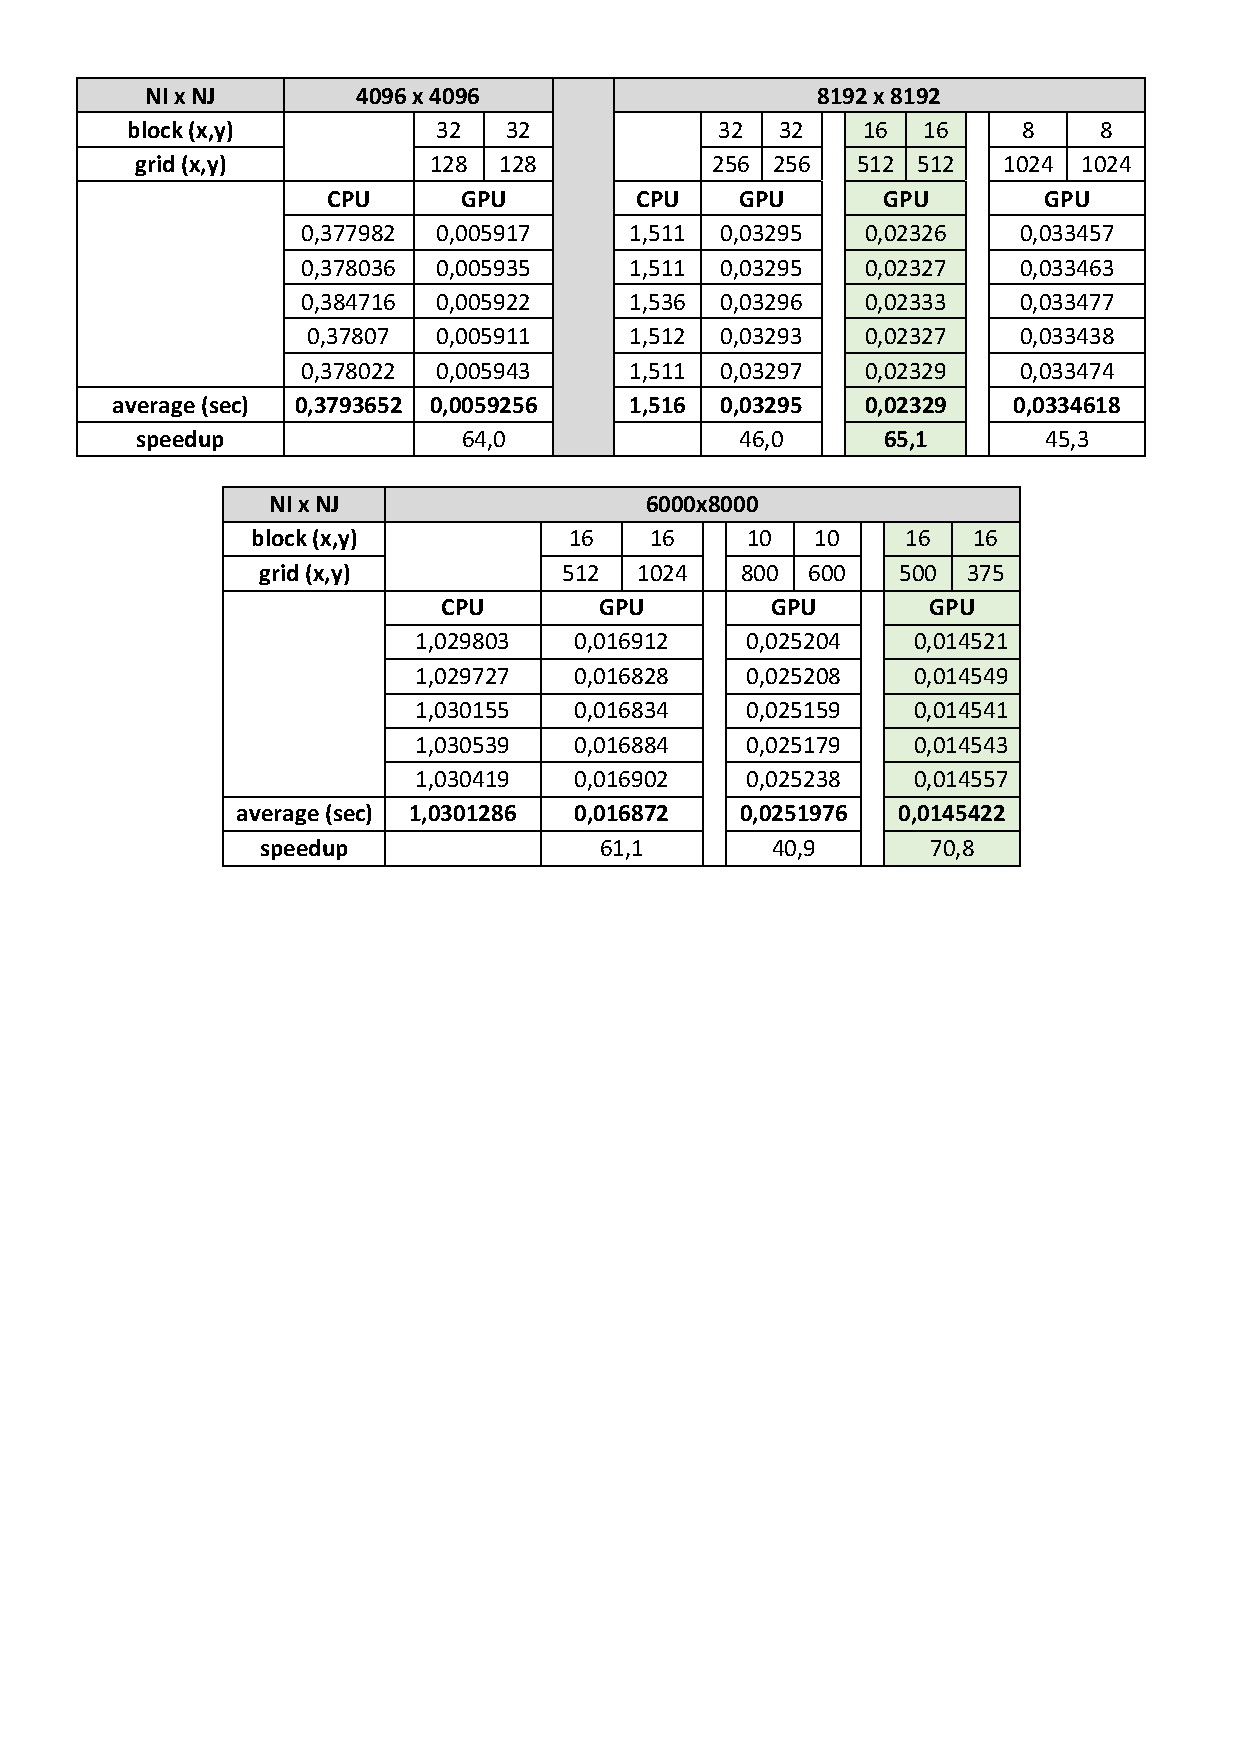
\includegraphics[scale=0.8]{./figures/1_conv/table1}
\end{center}

Ιδιαίτερο ενδιαφέρον παρουσιάζει η περίπτωση στην οποία το μέγεθος του μητρώου είναι 6000Χ8000, ένα grid αρκετά μεγαλύτερο από το μητρώο δίνει σημαντικά καλύτερη απόδοση από ένα άλλο grid με διαστάσεις που ενώ  ταιριάζουν ακριβώς στο αρχικό μητρώο, δεν έχουν μέγεθος block πολλαπλάσιο του warp size. Σε κάθε περίπτωση καλύτερη απόδοση επιτυγχάνουμε όταν για 16×16 block χρησιμοποιούμε το μικρότερο δυνατό grid. Αφού λοιπόν καταλήξαμε ότι στις περισσότερες περιπτώσεις block μεγέθους 16×16 μας δίνουν την καλύτερη συμπεριφορά μπορούμε να εκφράσουμε αλγοριθμικά τον υπολογισμό του απαιτούμενου μεγέθους για το grid ανάλογα με το μέγεθος της εισόδου (NI, NJ) ως εξής:

\vspace{0.3cm}

\newpage

\begin{lstlisting}[language=C]
    // given block size
	int block_dim_x = 16;
	int block_dim_y = 16;

	// calculate grid dimensions
	int grid_dim_x = ceil( (float) NJ / block_dim_x );
	int grid_dim_y = ceil( (float) NI / block_dim_y );
\end{lstlisting}

\begin{center}
    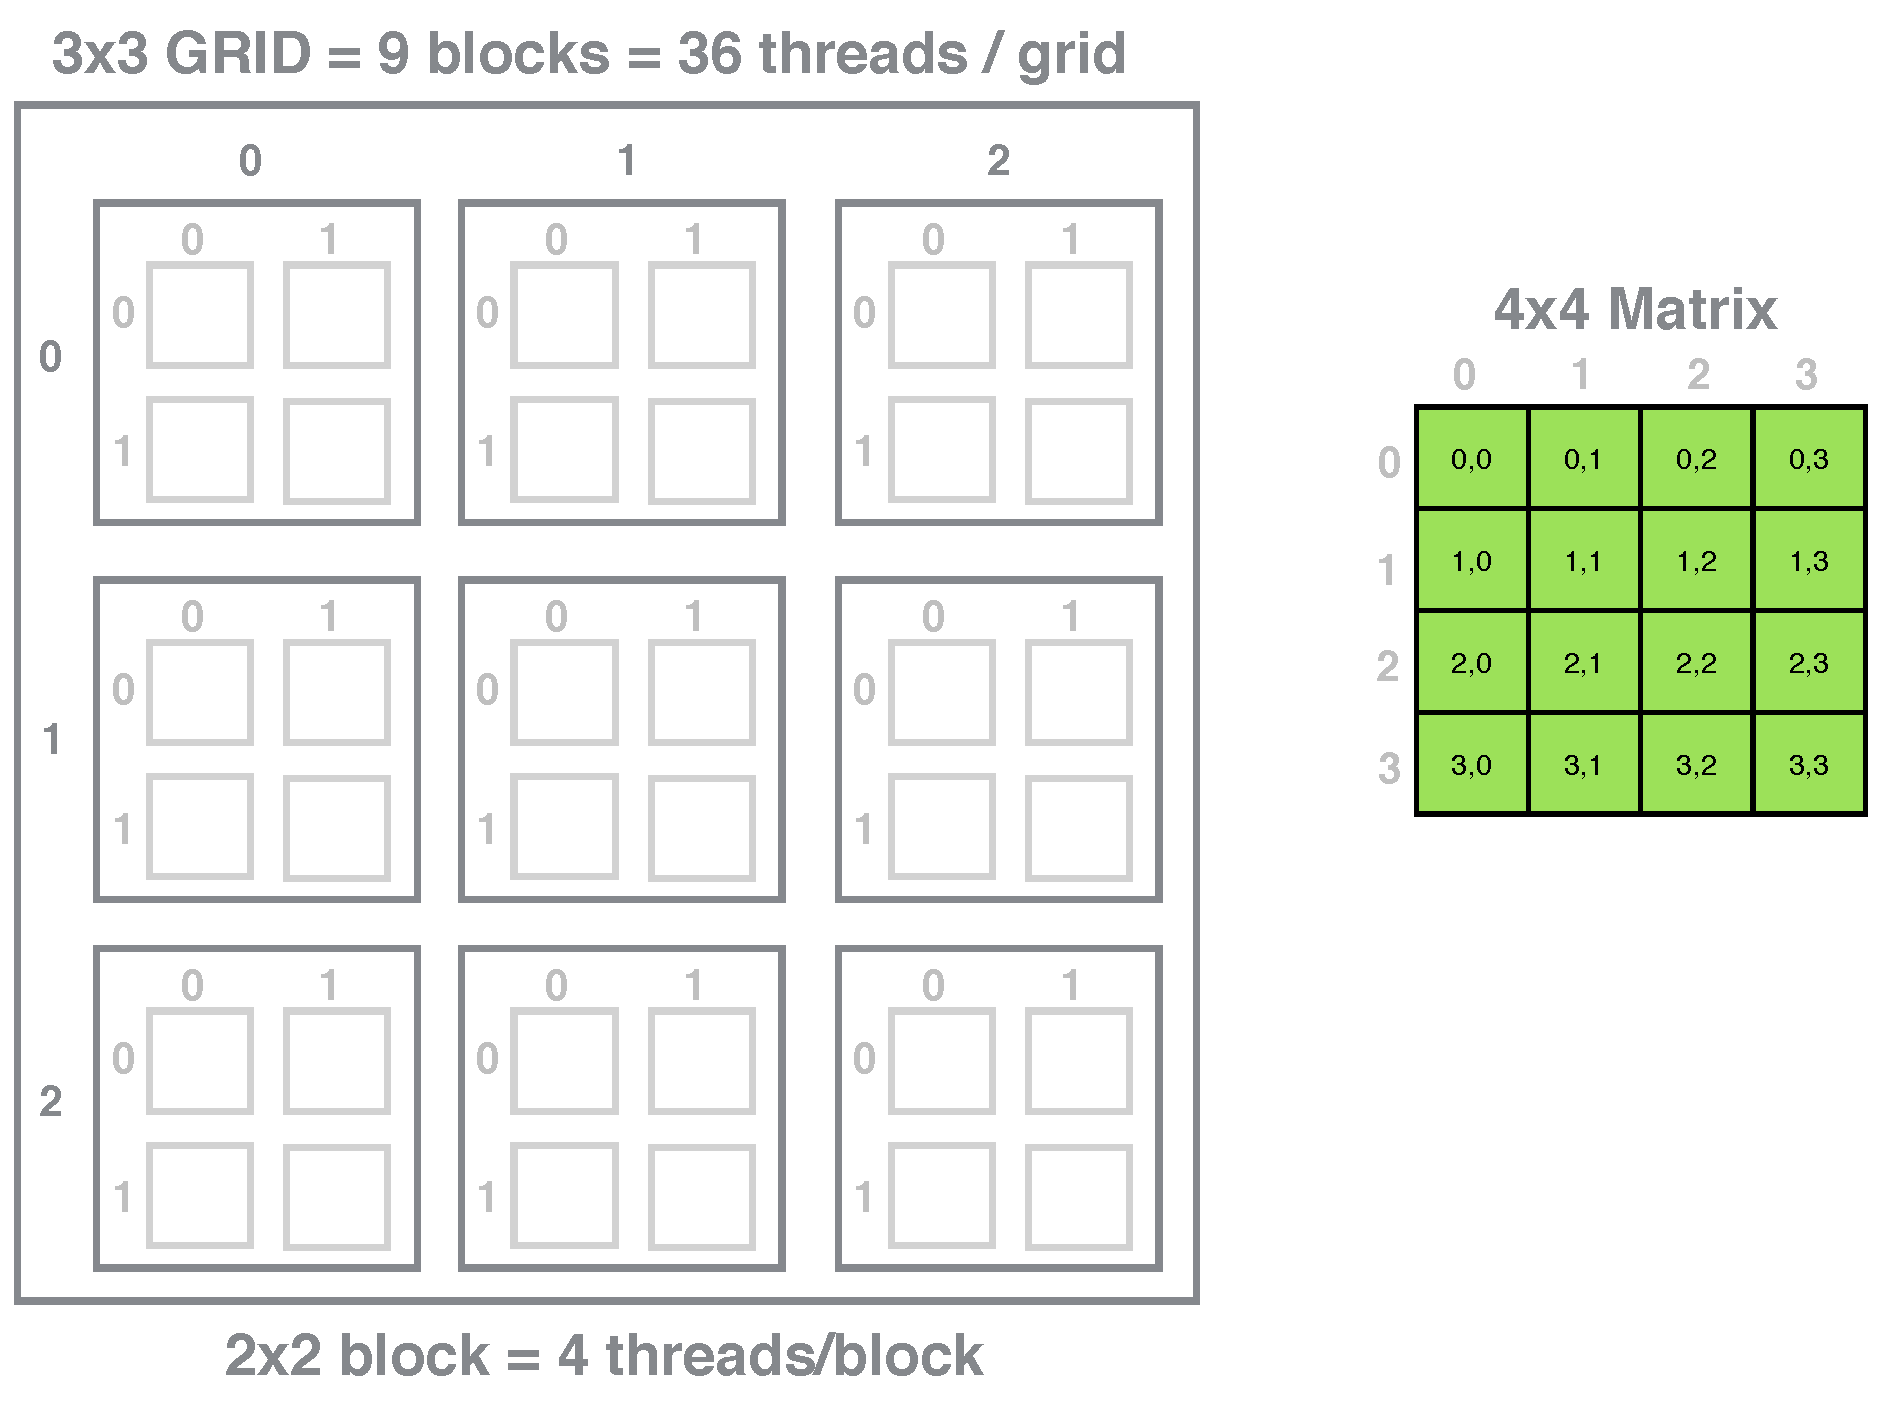
\includegraphics[scale=0.35]{./figures/1_conv/grid-matrix}
\end{center}

\begin{center}
    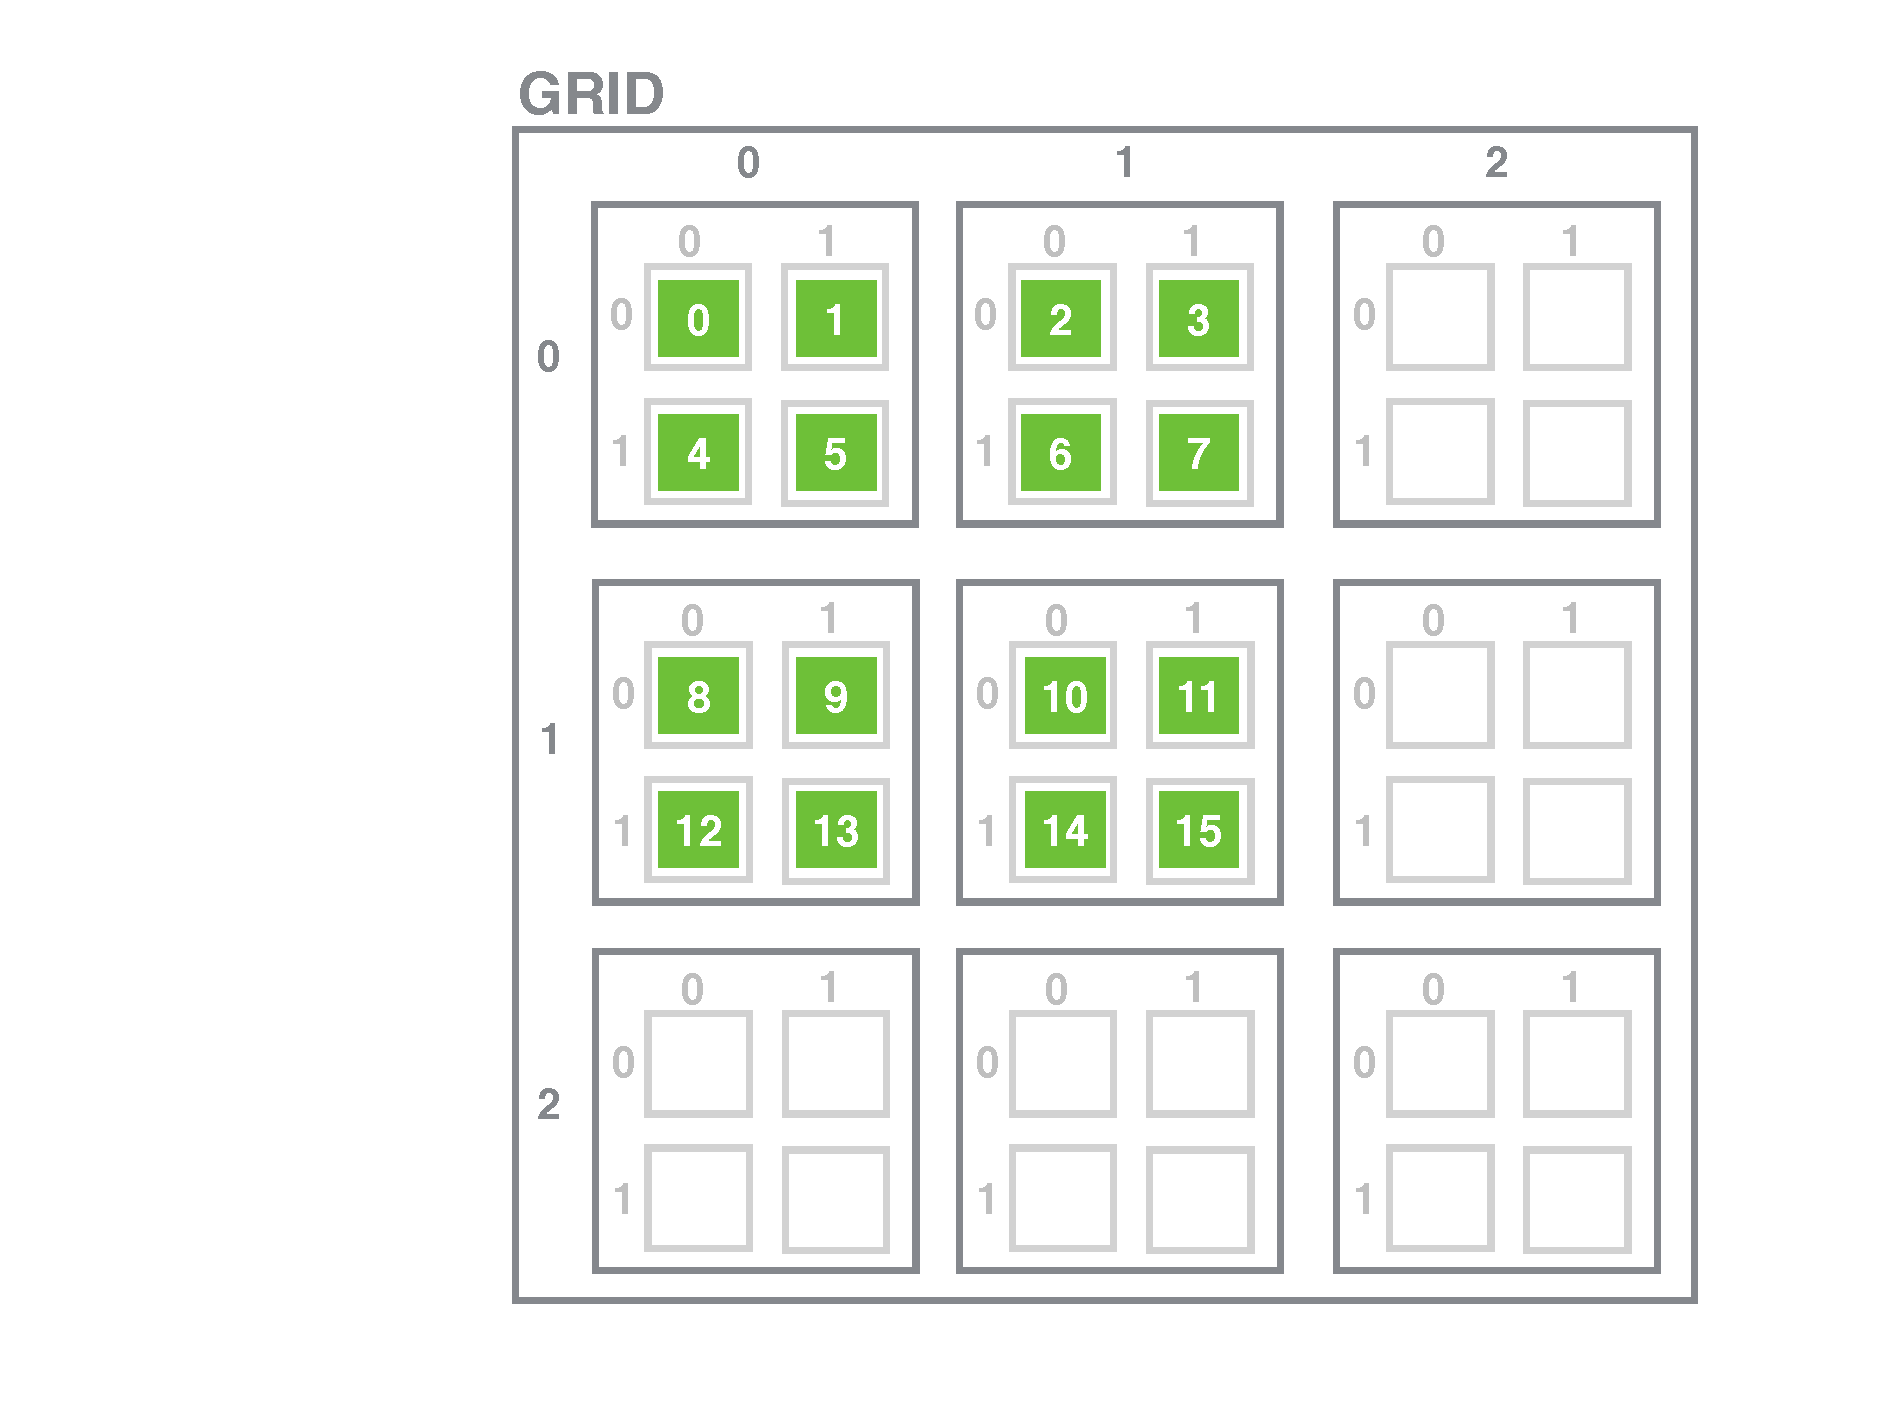
\includegraphics[scale=0.35]{./figures/1_conv/final-grid}
\end{center}

Στο παραπάνω σχήμα φαίνεται ο τρόπος με τον οποίο αντιστοιχούμε ένα 4x4 μητρώο σε δεδομένων διαστάσεων grid, μέσω της μονοδιάστατης αναπαράστασής του στην μνήμη. Στην πραγματικότητα βέβαια τα πράγματα είναι διαφορετικά αφού δεν χρησιμοποιούμε προκαθορισμένες διαστάσεις για το grid αλλά ο αριθμός των block καθορίζεται δυναμικά ώστε να είναι ο ελάχιστος απαραίτητος σε κάθε διάσταση.

\newpage